\documentclass[tikz,border=5pt]{standalone}
\usepackage[UTF8]{ctex}
\usepackage{amsmath,amssymb}
\usetikzlibrary{arrows.meta,calc,angles,quotes,patterns,decorations.pathmorphing}
\definecolor{field}{HTML}{176B9B}
\definecolor{force}{HTML}{B64B32}
\tikzset{>=Latex,line width=.8pt,every node/.style={font=\small},field/.style={color=field},force/.style={color=force},body/.style={draw=black,fill=blue!5},ghost/.style={dashed,gray},labelbox/.style={fill=white,inner sep=1.2pt}}
\begin{document}
\begin{tikzpicture}
\draw[thick](-2.4,0)--(3,0)node[right]{地面};
\draw[body](0,3.3)circle(1.1);
\draw[ghost](-1.1,3.3)arc(180:0:1.1 and .3);
\draw(-1.1,3.3)arc(180:360:1.1 and .3);
\draw[ghost](0,2.2)arc(270:90:.35 and 1.1);
\draw(0,2.2)arc(270:450:.35 and 1.1);
\draw[->](0,3.3)--(.78,4.08)node[midway,above left]{$r$};
\node[labelbox]at(0,3.1){$\rho_{\rm i},T_{\rm i},p_{\rm i}$};
\draw[<->](-1.7,0)--(-1.7,1.1);
\draw[<->](-1.7,1.5)--(-1.7,3.3);
\draw(-1.8,1.2)--(-1.6,1.3)--(-1.8,1.4);
\node[left]at(-1.7,2.5){$h$};
\node[right]at(1.4,3.5){$\rho_h,T_h,p_h$};
\node[below]at(.1,-.45){高度轴截断；气囊体积固定};
\end{tikzpicture}
\begin{tikzpicture}
\begin{scope}
\draw[body](0,.8)rectangle(2.3,1.8);
\draw[->,field](.6,.2)--(.6,.8)node[midway,left]{$pS$};
\draw[->,field](1.5,2.5)--(1.5,1.8)node[midway,right]{$(p+{\rm d}p)S$};
\draw[->,force](1.15,1.3)--(1.15,.8)node[below right]{$\rho gS\,{\rm d}z$};
\draw[<->](2.7,.8)--(2.7,1.8)node[midway,right]{$ {\rm d}z$};
\end{scope}
\begin{scope}[xshift=5cm,x=1.5cm]
\draw[->](0,0)--(2,0)node[right]{相对降幅 $\times100$};
\draw[->](0,0)--(0,3.6)node[above]{$z/h$};
\draw[field,thick](0,0)--(1.5401485,3);
\draw[force,thick](0,0)--(1.1001061,3);
\draw[green!50!black,thick](0,0)--(.4400424,3);
\node[above]at(1.5401485,3){$p$};\node[above]at(1.1001061,3){$\rho$};
\node[above]at(.4400424,3){$T$};\node[left]at(0,3){$1$};
\draw(1,0)--(1,-.08)node[below]{$1$};
\end{scope}
\end{tikzpicture}
\begin{tikzpicture}
\draw[body](0,0)rectangle(3,2.2);
\node[align=center]at(1.5,1.3){定容 $V$\\$n,T,p$};
\draw[very thick](3,1)--(3.5,1);
\draw[->,force,thick](3.5,1)--(5,1)node[right]{$-{\rm d}n>0$};
\node[force,above]at(4.3,1.2){$C_PT(-{\rm d}n)$};
\node[below]at(1.5,-.6){$Q=0$，流出气体携带焓};
\draw[->](3,2.8)--(6.7,2.8)node[midway,above]{随后关闭出口};
\draw[body](6.7,0)rectangle(9.7,2.2);
\node[align=center]at(8.2,1.3){封闭定容\\$n_{\rm b},T_{\rm b},p_{\rm b}$};
\draw[thick](9.7,.7)--(9.7,1.3);
\node[below]at(8.2,-.6){升空时质量固定};
\end{tikzpicture}
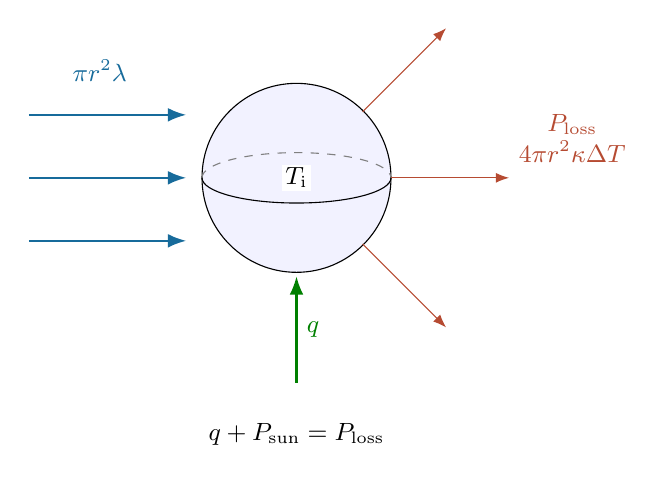
\begin{tikzpicture}
\draw[body](0,0)circle(1.2);
\draw[ghost](-1.2,0)arc(180:0:1.2 and .32);
\draw(-1.2,0)arc(180:360:1.2 and .32);
\foreach\y in{-.8,0,.8}\draw[->,field,thick](-3.4,\y)--(-1.4,\y);
\node[field,above]at(-2.5,1.1){$\pi r^2\lambda$};
\draw[->,force](1.2,0)--(2.7,0);
\draw[->,force](.84,.84)--(1.9,1.9);
\draw[->,force](.84,-.84)--(1.9,-1.9);
\node[force,right,align=center]at(2.7,.5){$P_{\rm loss}$\\$4\pi r^2\kappa\Delta T$};
\draw[->,green!50!black,thick](0,-2.6)--(0,-1.25)node[midway,right]{$q$};
\node[labelbox]at(0,0){$T_{\rm i}$};
\node[below]at(0,-3){$q+P_{\rm sun}=P_{\rm loss}$};
\end{tikzpicture}
\begin{tikzpicture}
\draw[body](-1.5,2)rectangle(1.5,2.8);\node at(0,2.4){热汇 $T_{\rm i}$};
\draw[body](-1.5,-2.8)rectangle(1.5,-2);\node at(0,-2.4){冷源 $T_h$};
\draw[body](0,0)circle(.65);\node at(0,0){热泵};
\draw[->,force,thick](0,.65)--(0,2)node[midway,right]{$q$};
\draw[->,field,thick](0,-2)--(0,-.65)node[midway,right]{$q_{\rm c}$};
\draw[->,thick](-2.5,0)--(-.65,0)node[midway,above]{$W$};
\node[right,align=left]at(2,0){$q=q_{\rm c}+W$\\[4pt]$\frac q{T_{\rm i}}\geq\frac{q_{\rm c}}{T_h}$};
\end{tikzpicture}
\end{document}
